\item \points{15} {\bf Kernelizing the Perceptron}

Let there be a binary classification problem with $y \in \{0, 1\}$.  The
perceptron uses hypotheses of the form $h_\theta(x) = g(\theta^T x)$, where
$g(z) = \text{sign}(z) = 1$ if $z \ge 0$, $0$ otherwise.  In this problem we
will consider a stochastic gradient descent-like implementation of the
perceptron algorithm where each update to the parameters $\theta$ is made using
only one training example.  However, unlike stochastic gradient descent, the
perceptron algorithm will only make one pass through the entire training set.
The update rule for this version of the perceptron algorithm is given by
\begin{equation*}
  \theta^{(i+1)} :=
	  \theta^{(i)} + \alpha (y^{(i+1)} - h_{\theta^{(i)}}(x^{(i+1)})) x^{(i+1)}
\end{equation*}
where $\theta^{(i)}$ is the value of the parameters after the algorithm has
seen the first $i$ training examples. Prior to seeing any training examples,
$\theta^{(0)}$ is initialized to $\vec{0}$.

\begin{enumerate}
  \item \subquestionpoints{3} Let $K$ be a kernel corresponding to some
very high-dimensional feature
mapping $\phi$. Suppose $\phi$ is so high-dimensional (say,
$\infty$-dimensional) that it's infeasible to ever represent $\phi(x)$
explicitly.  
Describe how you would apply the ``kernel trick'' to the
perceptron to make it work in the high-dimensional feature space $\phi$, but
without ever explicitly computing $\phi(x)$.

[\textbf{Note:} You don't have to worry about the intercept term.  If you like,
think of $\phi$ as having the property that $\phi_0(x) = 1$ so that this is
taken care of.] Your description should specify:
\begin{enumerate}[label=\roman*.]
  \item \subquestionpoints{1} How you will (implicitly) represent the
  high-dimensional
    parameter vector $\theta^{(i)}$, including how the initial value
    $\theta^{(0)} = 0$ is represented (note that $\theta^{(i)}$ is
    now a vector whose dimension is the same as the feature vectors
    $\phi(x)$);
  \item \subquestionpoints{1} How you will efficiently make a prediction on a
  new input
    $x^{(i+1)}$.  I.e., how you will compute
    $h_{\theta^{(i)}}(x^{(i+1)}) = g({\theta^{(i)}}^T \phi(x^{(i+1)}))$,
    using your representation of $\theta^{(i)}$; and
  \item \subquestionpoints{1} How you will modify the update rule given above
  to perform an
  update to $\theta$ on a new training example $(x^{(i+1)}, y^{(i+1)})$;
  \emph{i.e.,} using the update rule corresponding to the feature mapping
  $\phi$:
  \begin{equation*}
  \theta^{(i+1)} :=
	  \theta^{(i)} + \alpha (y^{(i+1)} - h_{\theta^{(i)}}(x^{(i+1)})) \phi(x^{(i+1)})
  \end{equation*}
\end{enumerate}


\ifnum\solutions=1 {
  \begin{answer}

  Note: For this question students were allowed to choose two different parameterizations for y. They could do $y \in \{0, 1\}$ or $y \in \{-1, 1\}$.
  Each paramaterization should result in slightly different answers. Both should be graded as correct.

  In the high-dimensional space we update $\theta$ as follows:
  \[ \theta := \theta + \alpha(y^{(i)} - h_\theta(\phi(x^{(i)})))
  \phi(x^{(i)}) \]

  So (assuming we initialize $\theta^{(0)} = \vec{0}$) $\theta$ will always be
  a linear combination of the $\phi(x^{(i)})$, i.e., $\exists \beta_l$
  such that $\theta^{(i)} = \sum_{l=1}^i \beta_l \phi(x^{(l)})$ after having
  incorporated $i$ training points.  Thus $\theta^{(i)}$ can be compactly
  represented by the coefficients $\beta_l$ of this linear
  combination, i.e., $i$ real numbers after having incorporated $i$
  training points $x^{(i)}$.  The initial value $\theta^{(0)}$ simply
  corresponds to the case where the summation has no terms (i.e., an empty list
  of coefficients $\beta_l$).

  We do not work explicitly in the high-dimensional space, but use the
  fact that
  $$
  g({\theta^{(i)}}^T \phi(x^{(i+1)}))
  = g(\sum_{l=1}^i \beta_l \cdot \phi(x^{(l)})^T \phi(x^{i+1}))
  = g(\sum_{l=1}^i \beta_l K(x^{(l)}, x^{(i+1)})),
  $$
  which can be computed efficiently.

  We can efficiently update $\theta$. We just need to compute $\beta_i
  = \alpha(y^{(i)} - g({\theta^{(i-1)}}^T \phi(x^{(i)})))$ at iteration $i$.
  This can be computed efficiently, if we compute ${\theta^{(i-1)}}^T
  \phi(x^{(i)})$ efficiently as described above.

  In an alternative approach, one can observe that, unless a sample
  $\phi(x^{(i)})$ is misclassified, $y^{(i)} - h_{\theta^{(i)}}(
  \phi(x^{(i)}) )$ will be zero; otherwise, it will be $\pm 1$ (or $\pm 2$, if
  the convention $y, h \in \{-1, 1\}$ is taken). The vector $\theta$, then, can
  be represented as the sum
  $\sum_{ \{ i : y^{(i)} \ne h_{\theta^{(i)}}( \phi(x^{(i)}) ) \} }
  \alpha (2y^{(i)} - 1) \phi(x^{(i)})$ under the $y,h \in \{0,1\}$ convention,
  and containing $(2 y^{(i)})$ under the other convention. This can then be
  expressed as $\theta^{(i)} = \sum_{i \in \text{Misclassified} } \beta_i
  \phi(x^{(i)})$ to be in more obvious congruence with the above. The efficient
  representation can now be said to be a list which stores only those indices
  that were misclassified, as the $\beta_i$s can be recomputed from the
  $y^{(i)}$s and $\alpha$ on demand. The derivation for (b) is then only
  cosmetically different, and in (c) the update rule is to add $(i+1)$ to the
  list if $\phi(x^{(i+1)})$ is misclassified.
\end{answer}

} \fi

  \item \subquestionpoints{10} Implement your approach by completing the
\texttt{initial\_state}, \texttt{predict}, and \texttt{update\_state} methods
of \texttt{src/perceptron/perceptron.py}.


We provide three functions to be used as kernel, a dot-product kernel defined as:
\begin{align}
	K(x,z) = x^\top z,
\end{align}
a
radial basis function (RBF) kernel, defined as:
\begin{align}
K(x,z) = \exp \left (-\frac{\|x-z\|_2^2}{2\sigma^2}\right), 
\end{align}
and finally the following function:
\begin{align}
K(x,z) = \begin{cases}
	 -1 & x=z \\
	 0 & x\neq z
	\end{cases}
\end{align}
\sloppy Note that the last function is not a kernel function (since its corresponding matrix is not a PSD matrix).
However, we are still interested to see what happens when the kernel is invalid.
%
 Run \texttt{src/perceptron/perceptron.py} to train
kernelized perceptrons on \texttt{src/perceptron/train.csv}. The code will then test
the perceptron on \texttt{src/perceptron/test.csv} and save the resulting
predictions in the \texttt{src/perceptron/} folder. Plots will also be saved in
\texttt{src/perceptron/}.


Include the three plots (corresponding to each of the kernels) in your writeup,
and indicate which plot belongs to which function.


\ifnum\solutions=1 {
  \begin{answer}
	\begin{figure}[H]
		\centering
		\vspace{-2mm}
		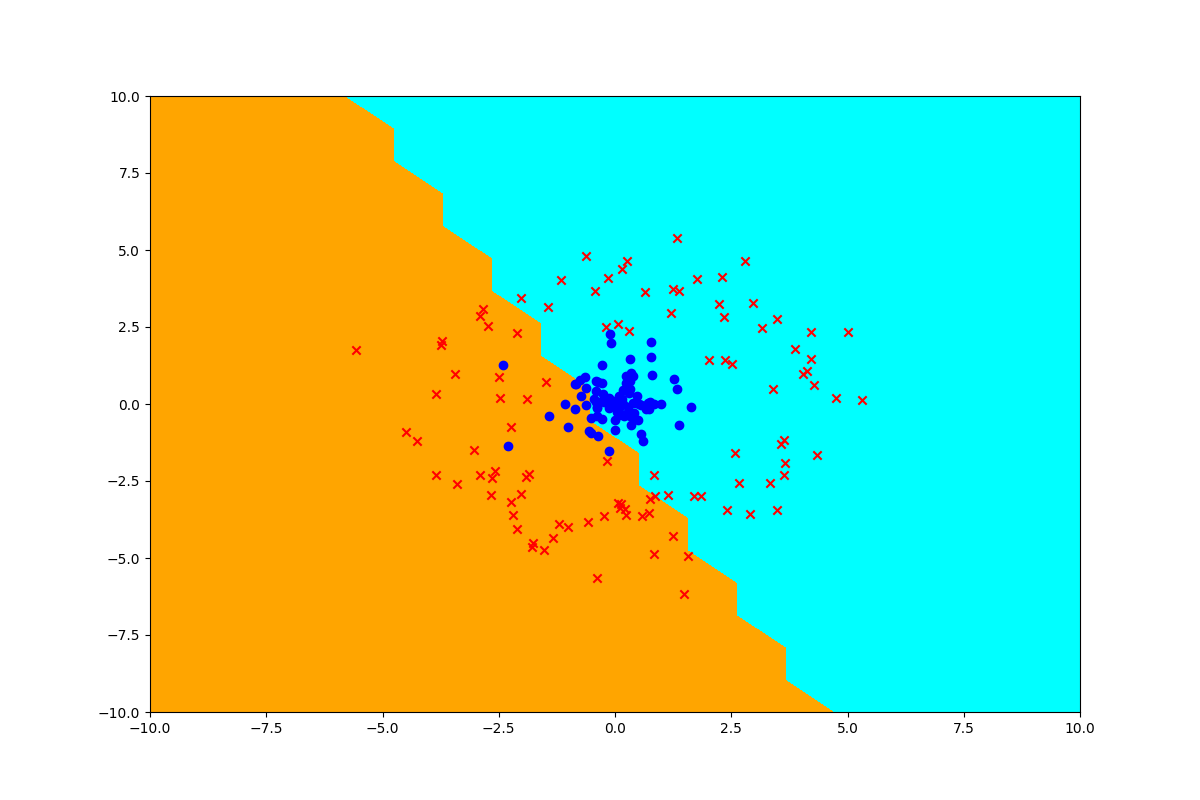
\includegraphics[width=0.65\linewidth]{../src/perceptron/perceptron_dot_output.png}
		\caption{Perceptron classifier plot for dot-product kernel}
		\centering

		\vspace{2mm}
		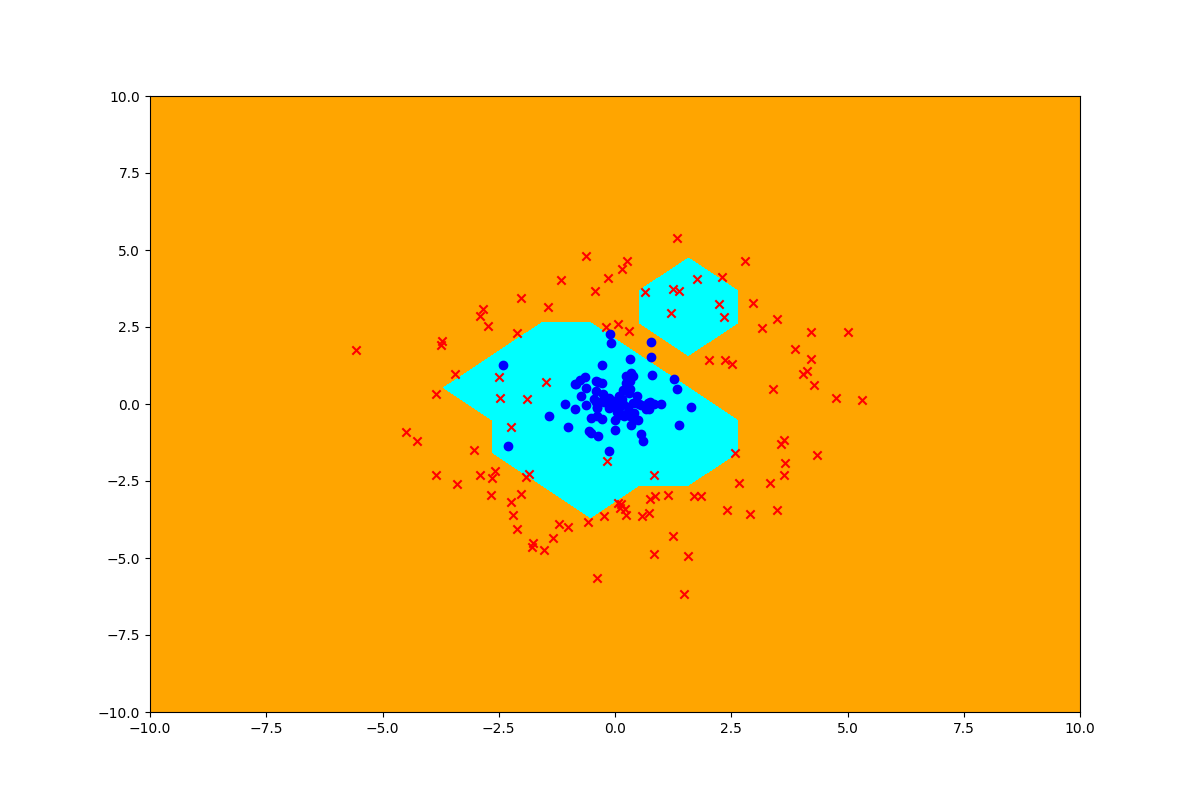
\includegraphics[width=0.65\linewidth]{../src/perceptron/perceptron_rbf_output.png}
		\centering
	\caption{Perceptron classifier plot for radial basis function kernel}
	
			\centering
	
	\vspace{2mm}
	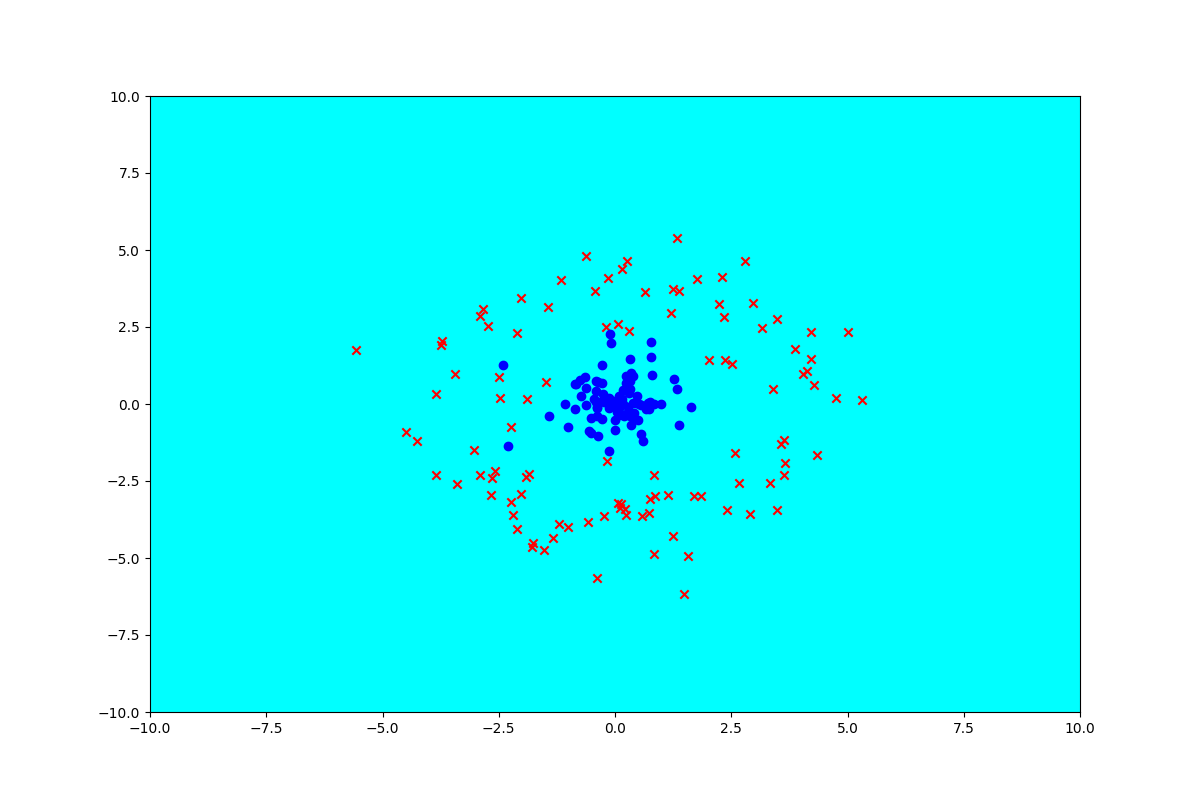
\includegraphics[width=0.65\linewidth]{../src/perceptron/perceptron_non_psd_output.png}
	\centering
	\caption{Perceptron classifier plot for the third choice}
	\end{figure}
\end{answer}

} \fi


  \item \subquestionpoints{2} 
One of the choices in Q4b completely fails, one works a bit, and one works well in classifying the points.
Discuss the performance of different choices and why do they fail or perform well?



\ifnum\solutions=1 {
  \begin{answer}
	The third choice fails completely since its corresponding matrix is not PSD; therefore, it is an invalid kernel function.
	It classifies all examples to the same class.
The dot product kernel performs badly as the data is not linearly separable.
Recall that kernels map $x$ to another feature space $\phi(x)$ but when we use dot-product kernel, we simply have $\phi(x)=x$; therefore, dot-product performs well when data is linearly separable.
\end{answer}

} \fi

\end{enumerate}
